%% Slides for ".NET Programming" by Chunyu Wang <chunyu@hit.edu.cn> %%

\part{C\# 语言基础}

\begin{frame}
\frametitle{Outline}            % {C\# 语言基础}
\tableofcontents
\end{frame}

\section{C\# 语言简介}

\begin{frame}
\frametitle{语言简介}

\begin{itemize}
    \setlength{\itemsep}{6pt plus 1pt}
\item C\# 是一种简洁、类型安全的面向对象的语言\par
\smallskip  \CJKindent 可以创建传统的 Windows 客户端应用程序、XML Web Services、分布式组
  件、客户端---服务器应用程序、数据库应用程序以及很多其他类型的程序。
\item 只有不到 90 个关键字
\item 支持泛型的方法和类型
\item 支持封装、继承和多态性概念
    % * 封装的方法签名(称为委托),它实现了类型安全的事件通知。
    % * 属性 (Property),充当私有成员变量的访问器。
    % * 属性 (Attribute),提供关于运行时类型的声明性元数据。
    % * 内联 XML 文档注释。
\item 支持指针和“不安全”代码的概念
\end{itemize}

\end{frame}


% \begin{frame}
% \frametitle{C\# 语言简介}
% \begin{itemize}
% \item 开发简单,功能强大,部署简单
% \item<1-| handout:1> 面向对象,一切皆为对象\\语言本身支持抽象类、接口、特性和事件等
% \item<2-| handout:1> 基于组件的开发\\提供内置的版本支持,接口与实现分离,事件的发布与订阅等
% \item<3-| handout:1> 与Web开发相结合\\可以将组件转变为Web服务,支持远程调用等
% \item<4-| handout:1> 更高的效率\\垃圾自动回收,变量是类型安全的,变量自动初始化等
% \item<4-| handout:1> 支持局部类、泛型等高级特性
% \end{itemize}
% \end{frame}

\note{
  \begin{itemize}
  \item C\#是一门较新的语言,在面向对象编成比较热的时候诞生,因此全面的支持面向
    对象开发。CTS 本身也是面向对象的系统
  \item 支持比较现代的软件开发的方法,组件开发
  \item 值得一提的是进行 Web Service 的开发
  \item 和 Java 类似,但优于Java,除支持垃圾自动回收等,还支持局部类泛型等
  \end{itemize}
}

% \section{C\#的基本语法}
\begin{frame}[fragile]
\frametitle{C\# 语言的语法}
\begin{itemize}
% \item 与 C 族语言类似(C/C++/Java)
%   \pause
\item 标识符区分大小,不能以数字开始
\item 变量可以随时声明,用 new 关键字创建类的实例
\begin{lstlisting}
int    a = 10;
Circle b = new Circle();
\end{lstlisting}
\item 注释有三种风格
\begin{lstlisting}
/* multi-line comments */
// single-line comments
/// <summary> XML comments </summary>
\end{lstlisting}
\item  通过XML注释,可自动生成程序文档
  \cmd{csc /doc:doc.xml source.cs}

\end{itemize}
\end{frame}

\note{
  \begin{itemize}
  \item 语法类似 C/C++/Java
  \item 同样的变量声明,创建类实例,如例子所示
  \end{itemize}
}

\begin{frame}[fragile]
\frametitle{C\# 程序示例}
\begin{itemize}
\item 所有程序逻辑和数据必须包含在类型中,没有全局变量

\item 通过 using 使用系统类库

\item 可执行文件必须有一个 \texttt{Main()} 方法,并用 \texttt{static} 修饰

\begin{lstlisting}
using System;
class MyFirstCSharpClass
{
  static void Main()
  {
    Console.WriteLine("A simple example");
    Console.ReadLine(); // read one char
    return;
  }
}
\end{lstlisting}

\end{itemize}
\end{frame}


\section{基本类型}

% \begin{frame}<0>
% \frametitle{基本数据类型  (\textit{Primitive Data Types})}
% \begin{tabular}{l|l|l}
% \hline
%   C\#类型 & FCL 类型       & 说明                 \\
% \hline
%   object  & System.Object  & 所有对象的基类型     \\
%   string  & System.String  & Unicode 字符序列     \\
%   bool    & System.Boolean & true 或 false       \\
%   char    & System.Char    & 字符型,2 字节       \\
%   byte    & System.Byte    & 单字节有符号整数     \\
%   sbyte   & System.SByte   & 单字节无符号整数     \\
%   short   & System.Int16   & 2 字节有符号整数     \\
%   ushort  & System.UInt16  & 2 字节无符号整数     \\
%   int     & System.Int32   & 4 字节有符号整数     \\
%   uint    & System.UInt32  & 4 字节无符号整数     \\
%   long    & System.Int65   & 8 字节有符号整数     \\
%   ulong   & System.UInt64  & 8 字节无符号整数     \\
%   float   & System.Single  & 单精度浮点数(4字节)  \\
%   double  & System.Double  & 双精度浮点数(8字节)  \\
%   decimal & System.Decimal & 高精度浮点数(16字节) \\
% \end{tabular}
% \end{frame}

\begin{frame}
\frametitle{基本操作符}
\begin{itemize}
\item 算数运算 \par
\texttt{$+,-,*,/,\%, +=,-=,*=,/=,++,--$}\par
指数运算操作符用\texttt{System.Math.Pow()}
\item 关系运算 \par
\texttt{$>, >=, <, <=, !=, ==$}
\item 逻辑运算 \par
\texttt{\&\&, ||, !}
\item 位运算 \par
\texttt{\&, |, \^}
\item 其他 \par
\texttt{?:}
\end{itemize}

\end{frame}


\begin{frame}
\frametitle{基本数据类型  (\textit{Primitive Data Types})}
\begin{itemize}
    \setlength{\itemsep}{8pt plus 1pt}
\item 布尔型:bool, 值为 true 或 false
\item 字符型:char, 长度为 2 字节的 Unicode 字符
\item 整数型:byte, sbyte, short, ushort, int, uint, long, ulong
\item 浮点型:float, double, decimal
\item 字符串型:string
%\item 引用型:object, reference
\item 枚举类型:enum
%\item 结构体型:struct
\end{itemize}
\end{frame}

\note{
  \begin{itemize}
  \item C\# 中有较丰富的数据类型
  \item 新的内置数据类型 string 和 bool,bool 长度为 1 字节,值为 true/false
  \item 分别支持 1/2/4/8 字节长的整型
  \item 以及 4/8/16 字节长的浮点型
  \end{itemize}
}

\begin{frame}[fragile]
\frametitle{C\# 类型与FCL 类型}
\begin{itemize}
\item C\# 的基本类型实际就是 FCL 类型的别名
\begin{lstlisting}
System.Int32 x = 100; // int x
int y = x;
\end{lstlisting}
\pause
\item 因此类型本身也由 FCL 提供了一些基本的成员和方法

\begin{lstlisting}
short smax = short.MaxValue;  //  32767
int   imin = int.MinValue;    // -2147483648

string s = "2372701";
int    v = int.Parse(s);

decimal z, y, pi = 3.14159265358979323846M;
y = decimal.Round(pi,3);        // 3.142
z = decimal.Remainder(pi,1.3M); // 0.54159265...

\end{lstlisting}
\end{itemize}
\end{frame}

\begin{frame}[fragile]
\frametitle{基本类型之间的转换}
\begin{itemize}
\item 数值之间
\begin{lstlisting}[escapeinside=<>]
int  i = 100;  long l = i;       // <隐式转换>
long l = 100;  int  i = (int) l; // <显示转换>
\end{lstlisting}
\pause
\item 与串之间
\begin{lstlisting}
int i = int.Parse("100");  string s =   i.ToString();
char c = char.Parse("A");  string s = 'A'.ToString();
\end{lstlisting}
\pause
\item 与字符之间
\begin{lstlisting}
int i = (int) '0';   // 0x30 or 48
char c = (char) 110; // 'n'
\end{lstlisting}
\end{itemize}
\end{frame}

\begin{frame}[fragile]
\frametitle{数据的表示}

\begin{itemize}
\item bool 只能有 \lstinline|true| 和 \lstinline|false| 两个值 \pause
\item 数字的后缀
  \begin{itemize}
    \lstset{emph={[3]L,M,U,UL,F}}
  \item \lstinline|100, 100U, 100L, 100UL; // int, uint, long, ulong|
  \item \lstinline|2.12F, 2.12, 2.12M;     // float, double, decimal|
  \end{itemize}
\pause
\item char 类型表示 Unicode 字符 (\lstinline| char c;|)
  \begin{columns}
    \column{.35\textwidth}
\begin{lstlisting}
c = 'B';
c = (char) 66;
c = '\u5B57';
c = '\x0042';
c = '\t';
c = char.Parse("K");
\end{lstlisting}
    \column{.55\textwidth}
\begin{lstlisting}
string s = "123abcd?";
char.IsLetter(s,3);
char.IsNumber(s,3);
char.IsLower(s,0);
char.IsPunctuation(s,7);
char.IsLetterOrDigit(s,1);
\end{lstlisting}
  \end{columns}
\end{itemize}
\end{frame}

\begin{frame}[fragile]
\frametitle{字符串}
% unicode 字符序列
\begin{itemize}
\item C\# 中基本的数据类型, Unicode 字符序列
\item 在堆中分配,但使用效果和值类型相似\pause
\item 使用 ``\texttt{@}'' 字符修饰,表示{\redwarn 逐字串}(\textit{Verbatim String})
\begin{lstlisting}
string s1, s2;
s1 =  "C:\\WINDOWS\\system32";
s2 = @"C:\WINDOWS\system32";

s1 =  "Hello \nWorld!";
s2 = @"Hello
World!";

s1 =  "cd \"Program Files\"";
s2 = @"cd ""Program Files""";
\end{lstlisting}
\end{itemize}
\end{frame}

\begin{frame}[fragile]
\frametitle{字符串的操作}
\begin{itemize}
\item 使用 ``\texttt{+}'' 可以直接连接串
\begin{lstlisting}
s1 = "Hello"; s2 = " World!";
s3 = s1 + s2 ;

s4 = "20.0/3 = " + 20.0/3;
// "20.0/3 = 6.66666666666667"
\end{lstlisting}

  \CJKindent \small 但需要注意,字符串的连接会生成新的串,如果大量操作,会影响
  效率,或用 System.Text.StringBuilder 。
\pause
\item 使用 ``=='' 判断是否相等
\begin{lstlisting}
string a = "abcdefgabcde";
string b = "abcdefgabcde";
Console.WriteLine(a==b); // Prints "True"
\end{lstlisting}
\end{itemize}
\end{frame}

\begin{frame}[fragile]
\frametitle{字符串的操作}
string 类型中提供的成员
\medskip
  \begin{itemize}
\setlength{\itemsep}{6pt plus 1pt}
  \item 查找字串 \texttt{IndexOf()}
  \item 比较字符串 \texttt{CompareTo(), Equals()}
  \item 转换大小写 \texttt{ToLower(), ToUpper()}
  % \item 对象的 ToString() 方法
  \item 串的长度 \texttt{Length}
  \end{itemize}
\begin{lstlisting}
string s = "This is a string";
int x = s.Length;
int y = "Hello World".Length;
\end{lstlisting}
\end{frame}

\begin{frame}[fragile]
\frametitle{字符串的操作}
抽取子串
\begin{lstlisting}
string s = "This is a string";
string t;

t = s.Substring(8); // "a string"
t = s.Substring(0,4); // "This"
\end{lstlisting}

定位子串
\begin{lstlisting}
string s = "This is a string";
int i;

i = s.IndexOf("a"); // i=8
\end{lstlisting}
\end{frame}

\begin{frame}[fragile]
\frametitle{格式化字符串}
\CJKindent
\begin{itemize}
\item 使用 ``\{N\}'' 表示后面参数次序
\begin{lstlisting}
string s1;
s1 = string.Format("Result is: {0}, {1}", 20, 3.22);
// "Result is: 20, 3.22"

\end{lstlisting}
\pause
\item 自定义的格式
\begin{lstlisting}
 s1 = string.Format("{0:0##.##}", 3.223); // "003.22"
 s1 = string.Format("{0:##%}", 0.45); // "45%"
\end{lstlisting}
\pause
\item 时间日期
\begin{lstlisting}
DateTime dt = DateTime.Now;
s1 = string.Format("{0:yyyy/MM/dd hh:mm:ss}", dt);
// "2005-05-12 11:40:22"
s1 = dt.ToString("yyyy-dd-MM");
\end{lstlisting}
\end{itemize}
\end{frame}

\begin{frame}[fragile]
\frametitle{结构体类型}
\CJKindent 结构体是和类(class)相似的一种简单的封装构造,同样可以包含成员变量和方法。
\begin{lstlisting}[escapeinside=<>]
struct Point {
  int x,y;
  public Point(int X, int Y)
    { x=X;  y=Y;}
}
\end{lstlisting}
\begin{itemize}
\item 结构体不能定义无参数的构造函数,不能定义析构函数
\item 如果定义构造函数,必须为结构体中的每个字段赋值
\end{itemize}
\end{frame}

\note{
  \begin{itemize}
  \item 也支持 struct,和 class 类似
  \end{itemize}}

\begin{frame}[fragile]
\frametitle{枚举类型}
枚举类型的一般格式
\begin{lstlisting}
[access modifiers] enum <identifier> [:enum-base]
{ body }
\end{lstlisting}

\begin{itemize}
    \setlength{\itemsep}{8pt plus 1pt}
\item 枚举类型
\begin{lstlisting}
enum Color
{Red, Blue=2, Green}

\end{lstlisting}

\item 改变枚举类型的默认整数
\begin{lstlisting}
enum Color:short
{Red=1, Blue=2, Green=3}
\end{lstlisting}
\end{itemize}
\end{frame}

\begin{frame}[fragile]
\frametitle{使用枚举}
\begin{itemize}
\item 枚举可以方便的创建常量
\item 可以提高程序的可读性
\item 枚举是一个类型,作为参数可以减少错误发生
\end{itemize}
\begin{lstlisting}
public int GetRGBValue(Color c){
  switch(c){
    case Color.Red:   return (0xFF0000);
    case Color.Green: return (0x00FF00);
    case Color.Blue:  return (0x0000FF);
  }
}
\end{lstlisting}

\end{frame}

\begin{frame}[fragile]
\frametitle{System.Enum 的方法}
System.Enum 是系统的枚举基类
\begin{itemize}
\item Enum.IsDefined() --- 判断字符串是否是某个枚举的成员
\item Enum.Parse() --- 解析字符串为枚举值
\item Enum.GetName() --- 通过枚举值返回枚举名字字符串
\end{itemize}
\begin{lstlisting}
  string s = "Green";
  if ( Enum.IsDefined( typeof(Color), s ) )
  {
    Color c =
      (Color) Enum.Parse (typeof(Color), s);

    Console.WriteLine ("Value 1 is: " +
      Enum.GetName (typeof (Color), 1));
  }
\end{lstlisting}
\end{frame}

\section{数组}

\begin{frame}[fragile]
\frametitle{数组}
声明数组的一般形式:
\begin{lstlisting}
<type><array_type> identifier
   = new <type><array_type> [{initializer list}]
\end{lstlisting}
\begin{itemize}
\item 数组类型可以是 ``\texttt{[]}'' ``\texttt{[,]}'' 或 ``\texttt{[][]}''
\item 可以省略初始化列表,默认值是 {\redwarn\texttt{0}} 或 {\redwarn\texttt{null}}
\item 也可以省略 new 表达式,直接通过列表定义
\end{itemize}
\pause
\begin{lstlisting}[escapeinside=<>]
int[] x; // <声明一个数组变量,默认值为 \texttt{null}>
int[] list = new int[5];
int[] list = new int[] {1,2,3,4,5}; // <初始化>
int[] list = {1,2,3,4,5}; //<short version>
\end{lstlisting}
\end{frame}

\begin{frame}[fragile]
\frametitle{数组}
\begin{itemize}
\item 一维数组,矩形多维数组 (\textit{Multidimensional Arrays})
\begin{lstlisting}[escapeinside=<>,mathescape]
int[] x = new int[5]; // <一维数组>

int[,] y = new int[2,5]; // $2\times5$ <二维数组>
\end{lstlisting}
\end{itemize} \pause

  \begin{figure}[h] \label<1| handout:1>{fig:cs-array-mul} \centering
    %% Slides for ".NET Programming" by Chunyu Wang <chunyu@hit.edu.cn> %% $Rev$

\begin{tikzpicture}[rounded corners, >=stealth]
\fill[yellow!40,fill opacity=.4] (0,-.1) rectangle +(8.5,4.45);
\draw (2.25,0) rectangle +(6,4.25);
\draw (.25,0) rectangle +(1.5,3);

\draw (5,3.75) node {�йܶ�} (1,2.75) node {�й�ջ};

\filldraw[fill=red!20, sharp corners] (.25, 1) rectangle +(1.5,.5) 
  (1,1.25) node {\footnotesize\texttt{x}};
\draw[->] (1.75, 1.25) .. controls +(right:.5cm) and +(left:.5cm) .. (2.5,1.25);

\fill[fill=blue!20,sharp corners,shift={(2.5,1)}] (0,0) rectangle +(1.5,2.5);
\draw[xstep=1.5cm,ystep=.5cm, sharp corners,shift={(2.5,1)}] (0,0) grid +(1.5,2.5);

\foreach \a in {0,1,...,4}
\draw  (3.25,1.25) +(0cm, .5cm*\a) node {\footnotesize\texttt{x[\a]}};



\filldraw[fill=red!20, sharp corners] (.25, .5) rectangle +(1.5,.5) 
  (1,.75) node {\footnotesize\texttt{y}};
\draw[->] (1.75, .75) .. controls +(-30:1cm) and +(210:1cm) .. (4.5,.75);

\fill[fill=blue!20,sharp corners,shift={(4.5,.5)}] (0,0) rectangle +(3,2.5);
\draw[xstep=1.5cm,ystep=.5cm, sharp corners,shift={(4.5,.5)}] (0,0) grid +(3,2.5);

\foreach \a in {0,1,...,4}
\draw  (5.25,.75) +(0cm, .5cm*\a) node {\footnotesize\texttt{y[0,\a]}};
\foreach \a in {0,1,...,4}
\draw  (6.75,.75) +(0cm, .5cm*\a) node {\footnotesize\texttt{y[1,\a]}};
\end{tikzpicture}

  \end{figure}
\end{frame}

\note{
  \begin{itemize}
  \item 数组的声明稍有不同,不过和 Java 类似
  \item int[]表示类型,需要创建实例
  \item int[,] 和 int[][]不同
  \end{itemize}
}

\begin{frame}[fragile]
\frametitle{多维数组}
\begin{itemize}
\item 锯齿形多维数组 (\textit{Jagged Arrays})
\begin{lstlisting}[escapeinside=<>]
int[][] z = new int[3][];
     z[0] = new int[4]; // z[0]<长度为4>
     z[1] = new int[3]; // z[1]<长度为3>
     z[2] = new int[5]; // z[2]<长度为5>
//z[0]<只是数组变量;>z[0][0]<才是整数>

\end{lstlisting}
\end{itemize} \pause

  \begin{figure}[h] \label<1| handout:1>{fig:cs-array-rec}
    \centering %% Slides for ".NET Programming" by Chunyu Wang <chunyu@hit.edu.cn>
%% $Rev$ $LastChangedDate$

\begin{tikzpicture}[rounded corners, >=stealth]
\fill[yellow!40,fill opacity=.4] (0,-.1) rectangle +(8.5,4.45);
\draw (2.25,0) rectangle +(6,4.25);
\draw (.25,0) rectangle +(1.5,3);

\draw (5,3.75) node {�йܶ�} (1,2.75) node {�й�ջ};

\fill[fill=blue!20,sharp corners,shift={(2.5,1.5)}] (0,0) rectangle +(1.5,2);
\fill[fill=blue!20,sharp corners,shift={(4.5,1.5)}] (0,0) rectangle +(1.5,1.5);
\fill[fill=blue!20,sharp corners,shift={(6.5,1.5)}] (0,0) rectangle +(1.5,2.5);
\fill[fill=red!20,sharp corners,shift={(3,.25)}]    (0,0) rectangle +(4.5,.5);

\draw[xstep=1.5cm,ystep=.5cm, sharp corners,shift={(2.5,1.5)}] (0,0) grid +(1.5,2);
\draw[xstep=1.5cm,ystep=.5cm, sharp corners,shift={(4.5,1.5)}] (0,0) grid +(1.5,1.5);
\draw[xstep=1.5cm,ystep=.5cm, sharp corners,shift={(6.5,1.5)}] (0,0) grid +(1.5,2.5);
\draw[xstep=1.5cm,ystep=.5cm, sharp corners,shift={(3,.25)}]   (0,0) grid +(4.5,.5);

\foreach \a/\b in {3.75/3.25, 5.25/5.25, 6.75/7.25}
\draw[->] (\a,.75) .. controls +(up:.5cm) and +(down:.5cm) .. (\b,1.5);

\filldraw[fill=red!20, sharp corners] (.25, .75) rectangle +(1.5,.5) 
  (1,1) node {\footnotesize\texttt{z}};
\draw[->] (1.75, 1) .. controls +(right:.5cm) and +(left:.5cm) .. (3,.5);

\foreach \a/\b in {3.75/z[0], 5.25/z[1], 6.75/z[2]} 
\draw (\a,.5) node {\footnotesize\texttt{\b}};

\foreach \a in {0,1,...,3}
\draw  (3.25,1.75) +(0cm, .5cm*\a) node {\footnotesize\texttt{z[0][\a]}};
\foreach \a in {0,1,...,2}
\draw  (5.25,1.75) +(0cm, .5cm*\a) node {\footnotesize\texttt{z[1][\a]}};
\foreach \a in {0,1,...,4}
\draw  (7.25,1.75) +(0cm, .5cm*\a) node {\footnotesize\texttt{z[2][\a]}};
\end{tikzpicture}

  \end{figure}
\end{frame}

\begin{frame}[fragile]
\frametitle{数组的使用}
\texttt{System.Array} 是类库中数组类型的基类

\begin{itemize}
\item \texttt{Length} --- 数组的长度
\item \texttt{Clear()} --- 将数组清空 (0 或 null)
\item \texttt{Sort()} --- 将数组排序
\item \texttt{Reverse()} ---- 倒序排列
\item \texttt{Find()} --- 找到特定的元素
\end{itemize}
\begin{lstlisting}
char[] x = new char[] {'b', 'a', 'c'};
int    y = x.Length;
System.Array.Sort(x);
System.Array.Reverse(x);
\end{lstlisting}

\end{frame}

\begin{frame}[fragile]
\frametitle{溢出检查}
\begin{itemize}
\item 进行溢出检查
  \lstset{emph={checked,unchecked}}
\begin{lstlisting}[escapeinside=<>]
int i = 1000000, j = 1000000;
int x = checked(i*j);
//<发生运行时异常:>System.OverflowException

\end{lstlisting}

\item 不进行溢出检查
\begin{lstlisting}[escapeinside=<>]
int i = 1000000, j = 1000000;
int x = unchecked(i*j);
//<无异常出现,但> x=-727379968

\end{lstlisting}
\end{itemize}
\end{frame}


\begin{frame}[fragile]
\frametitle{预处理指令}
\begin{itemize}
\item 定义宏(\textit{macro}),检验宏\\

\texttt{\#define, \#undef, \#if, \#else, \#elif, \#endif}
\cmd{csc /Define:XX hello.cs}

\item 产生编译错误或警告

\texttt{\#error, \#warn}

\begin{lstlisting}
#if DEBUG && RELEASE
#error "DEBUG and RELEASE defined simultaneously"
#endif

#warning "Dont't forget TEST here"
\end{lstlisting}
\end{itemize}
\end{frame}

\begin{frame}[fragile]
\frametitle{预处理指令}
\begin{itemize}
\item 定义代码段,用于 Visual Studio 的代码折叠

\texttt{\#region, \#endregion}

\begin{lstlisting}
#region Test Module
  ...
#endregion
\end{lstlisting}

\item 改变编译器当前的文件名和行号

\texttt{\#line}

\begin{lstlisting}
#line 123 "AnotherFile.cs"
  ...
#line default // restore
\end{lstlisting}
\end{itemize}

\end{frame}
\section{流程控制}

\begin{frame}[fragile]
\frametitle{分支语句}
  \begin{itemize}
  \item if-else 语句
\begin{lstlisting}
  if (a>=b){
    x =  1;
  } else if (a<b) {
    x = -1;
  }
\end{lstlisting}
  \item 判断条件的值必须是 \texttt{bool} 型的 \texttt{true} 或 \texttt{false}
\begin{lstlisting}[escapeinside=<>]
  int i = 1;
  if (i) { ... }
  // <编译错误:无法隐式的将int转为bool>
\end{lstlisting}
  \end{itemize}
\end{frame}

\begin{frame}[fragile]
\frametitle{分支语句}
  \begin{itemize}
  \item switch 语句
  \end{itemize}
  \begin{columns}
    \column{.5\textwidth}
\begin{lstlisting}
int Score; string r;
switch(Score/10){
  case 10:
  case 9:
    r = "A"; break;
  case 8:
    r = "B"; break;
  ...
  default:
    r = "E"; break;
}

\end{lstlisting}
    \column{.5\textwidth}
\begin{lstlisting}
int Score; string r;
switch(Score/10){
  case 10:
    r = "A+";
    goto case 9;
  case 9:
    r = "A"; break;
  ...
  default:
    r = "E"; break;
}

\end{lstlisting}
  \end{columns}
\end{frame}
\note{
  \begin{itemize}
  \item case 语句之间
  \item 如果语句为空,可以自动进入下一个 case 语句
  \item 如果不空必须显式使用 goto case xx; 语句
  \end{itemize}
}
\begin{frame}[fragile]
\frametitle{循环语句}
\begin{itemize}
\item while/do-while 循环
\begin{lstlisting}
while (condition) { ... }
do { ... } while (condition);
\end{lstlisting}
\item for 循环
\begin{lstlisting}
for(int i=0; i<5; i++) { ... }
\end{lstlisting}
  \pause
\item foreach 循环
\begin{lstlisting}
string[] colors={"Red","Green","Blue"};
foreach (string x in colors) {
  Console.WriteLine(x);
}
\end{lstlisting}
\begin{itemize}
\item foreach 循环对实现了IEnumerable$<$T$>$ 的对象进行迭代
\item 迭代中,对其中的对象只能只读访问
\end{itemize}
\end{itemize}
\end{frame}

\note{
  \begin{itemize}
  \item foreach 和 VB 中的类似,用来对数组中的每个元素进行迭代
  \item 使用 foreach 可以省去使用索引变量的麻烦,也不用判断数组的长度
  \end{itemize}
}

\begin{frame}[fragile]
\frametitle{foreach 与多维数组}
\begin{itemize}
\item foreach 对多维数组迭代,按行依次返回各元素
\item 不需要嵌套循环,不需要计算大小
\end{itemize}
\begin{lstlisting}
public static void Main() {
  int sum = 0;
  int[,] nums = new int[3,5];

  for(int i = 0; i < 3; i++)
    for(int j=0; j < 5; j++)
      nums[i,j] = (i+1)*(j+1);

  // use foreach to display and sum the values
  foreach(int x in nums) {
    Console.WriteLine("Value is: " + x);
    sum += x;
  }
\end{lstlisting}
\end{frame}


\begin{frame}
\frametitle{跳转语句}
\begin{itemize}
\item break \\用来退出循环或 swich 分支语句等
\item continue \\用来中断循环的当前迭代,并继续循环
\item goto \\任意跳转
\item return \\返回方法的调用
\end{itemize}
\end{frame}

%\section{异常}
\begin{frame}
\frametitle{错误处理}
\begin{itemize}
    \setlength{\itemsep}{8pt plus 1pt}
\item C\# 提供的标准处理方式---异常(\textit{Exception})
\item 捕捉和处理可能在运行时发生的错误的技术
\item C\# 中的异常就是一个对象,包含了错误的类型和详细信息
\item 异常能够给出调用栈的序列,用于分析异常发生的位置
\item 异常可以被捕获,并加以处理(C\# 的错误处理机制)
\item 异常可以分类,可以自己创建
\item 未被捕获的异常将提交给 CLR,并中止程序运行
\end{itemize}

\end{frame}

\begin{frame}[fragile]
\frametitle{异常处理}
\begin{itemize}
\item try 监测异常的发生
\begin{lstlisting}
try { ... }
\end{lstlisting}
\item catch 捕获并处理异常
\begin{lstlisting}[escapeinside=<>]
catch (SomeException e) {
  // <处理> SomeException <类型的异常> e
}

\end{lstlisting}
\item finally 确保必要操作一定会执行
\begin{lstlisting}
finally { ... }
\end{lstlisting}
\end{itemize}
\end{frame}

\note{
  \begin{itemize}
  \item 以一种优雅的方式处理错误
  \item 可以将正常代码和错误处理代码分开
  \end{itemize}}

\begin{frame}[fragile]
\frametitle{异常处理示例}
\begin{lstlisting}
// using System; using System.IO;
StreamWriter sw = null;
try {
  sw = new StreamWriter(
    new FileStream("T.txt",FileMode.Open));
  sw.WriteLine ("Hello World");
}
catch (FileNotFoundException e) {
  Console.WriteLine("File "
               +e.FileName+" not found.");
}
catch (Exception e){
  Console.WriteLine(e);
}
finally {
  if (sw!=null)   sw.Close();
}

\end{lstlisting}
\end{frame}

\begin{frame}[fragile]
\frametitle{抛出异常}
使用关键字 \texttt{throw} 向系统抛出异常。
\begin{lstlisting}
try {

  if (Overflow == true)
    throw new OverflowException();

  if (OutOfBounds == true)
    throw new IndexOutOfRangeException();

} catch (OverflowException e) {
   // error handling for overflow
} catch (IndexOutOfRangeException e) {
   // error handling for out of range
} finally {
   // clean up
}
\end{lstlisting}
\end{frame}

\note{
  \begin{itemize}
  \item 例子中打开文件处可能发生错误,如文件不存在,或者不可读
  \item 当不存在时,在第一个catch处捕获,并处理
  \item 其他任何错误,都会被更通用的异常类型捕获
  \item finally保证,无论是否发生异常,此处代码都会被执行
  \end{itemize}}

\begin{frame}
\frametitle{异常的分类}
\begin{columns}
  \column{.6\textwidth}
  \begin{itemize}
  \item Exception 继承自 Object,是异常系统的根
  \item SystemException 通常由 CLR 抛出
  \item ApplicationException 用于应用程序自定义异常
  \item 常见异常
    \begin{itemize}
    \item FileNotFoundException
    \item EndOfStreamException
    \item OverflowException
    \end{itemize}
  \end{itemize}
  \column{.4\textwidth}
  %% Slides for ".NET Programming" by Chunyu Wang <chunyu@hit.edu.cn> %%

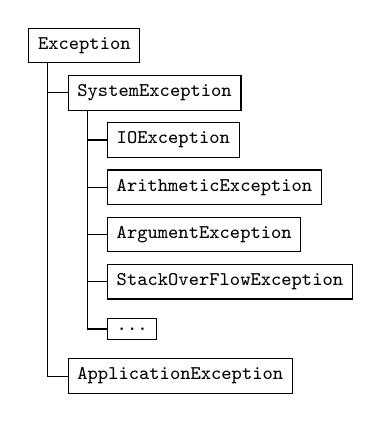
\begin{tikzpicture}
  \tikzstyle{every node}=[anchor=west, draw,fill=white, font=\ttfamily\scriptsize]
  \node at (0,5) (a) {Exception};
  \node at (.5,4.4) (b) {SystemException};
  \node at (1,3.8) (b1) {IOException};
  \node at (1,3.2) (b2) {ArithmeticException};
  \node at (1,2.6) (b3) {ArgumentException};
  \node at (1,2)   (b4) {StackOverFlowException};
  \node at (1,1.4) (b5) {\mbox{}...};
  \node at (.5,.8) (c) {ApplicationException};

  \draw (a.south west) +(right:.25cm) |- (b);
  \draw (a.south west) +(right:.25cm) |- (c);

  \foreach \a in {b1,b2,b3,b4,b5}
  \draw (b.south west) +(right:.25cm) |- (\a);
\end{tikzpicture}

\end{columns}
\end{frame}

% Local Variables:
% mode: LaTeX
% TeX-master: "part-02.tex"
% TeX-header-end: "% End-of-Header$"
% TeX-trailer-start: "% Start-of-Trailer$"
% coding: utf-8
% End:
